\section{Fourierfilterung}
\subsection{Ergebnis}
\subsection{Fourier Schriftzug}
Zuerst soll ein "Fourier" Schriftzug vor einem Gitter modelliert werden, indem das Gitter entfernt wird. Dazu wird eine Tiefpassfilterung benutzt, da die im Vergleich große Schrift hauptsächlich aus niedrigen Frequenzen besteht. 


\begin{figure}[h]
\begin{subfigure}[c]{0.5\textwidth}

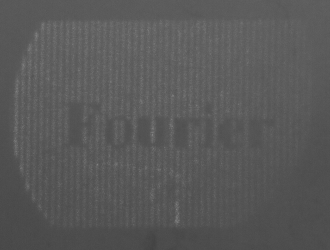
\includegraphics[width=0.9\textwidth]{Fourier.png}
	      \caption{}
          \label{fig:NiceImage1}
          
\end{subfigure}
\begin{subfigure}[c]{0.5\textwidth}
	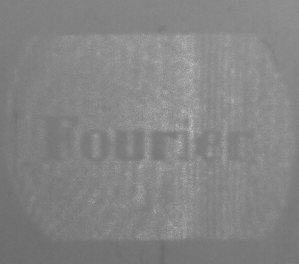
\includegraphics[width=0.9\textwidth]{Fourier_Filter.png}
	      \caption{}
          \label{fig:NiceImage2}
\end{subfigure}
\caption{In \cref{fig:NiceImage1} ist der "Fourier" Schriftzug ohne Filter zu sehen; in \cref{fig:NiceImage2} mit einem Tiefpassfilter.}
\label{Fourier}
\end{figure}   

In \cref{Fourier} ist zu sehen, wie sich der Tiefpassfilter auf das Bild auswirkt. Das Gitter ist zum größten Teil nicht mehr als solches zu erkennen.

\subsection{Nenner eines Bruches entfernen}
Daraufhin soll der Nenner eines $\frac{1}{2}$ Bruchs entfernt werden. Wie in \cref{fig:Bruch} zu sehen ist, befindet sich unter dem Zähler ein Gitter, welches sich nicht bei dem Nenner befindet. Es werden also praktisch beide Zahlen entfernt, allerdings ist durch das Gitter immer noch der Umriss der 1 sichtbar. Dieses entfernen geschieht durch eine Hochpassfilterung, was bedeutet, dass niedrige Frequenzen entfernt werden. Das hat sehr gut funktioniert, da in \cref{fig:Bruch_filter} die Zwei, also der Nenner nicht mehr erkennbar ist.

\begin{figure}[h]
	\begin{subfigure}[c]{0.5\textwidth}
		
		\includegraphics[width=0.6\textwidth]{Bruch.png}
		\caption{}
		\label{fig:Bruch}
		
	\end{subfigure}
	\begin{subfigure}[c]{0.5\textwidth}
		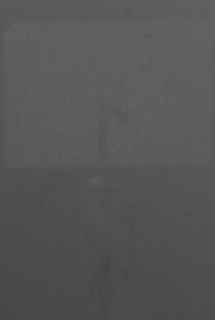
\includegraphics[width=0.58\textwidth]{Filter_Bruch.png}
		\caption{}
		\label{fig:Bruch_filter}
	\end{subfigure}
	\caption{In \cref{fig:Bruch} ist der $\frac{1}{2}$ Bruch ohne Filter zu sehen; in \cref{fig:Bruch_filter} mit einem Hochpassfilter, wodurch die Zwei entfernt wurde.}
	\label{Bruch}
\end{figure}   

\subsection{Tiefpassfilterung bei einem Quadratgitter}
Als nächstes soll ausprobiert werden, was passiert, wenn ein Quadratgitter eingesetzt wird, das mit einem eindimensionalem Tiefpassfilter in verschiedenen Ausrichtungen gefiltert wird. Das ungefilterte Bild ist in \cref{fig:Gitter} zu sehen. Dazu im Vergleich wurde in \cref{fig:0Gitter} ein Tiefpassfilter im Winkel von 0° Grad eingebaut. Da der Tiefpass alle Frequenzen außer denen, die im 0° Winkel sind durchgelassen. Deshalb wurde erwartet, dass die Linien orthogonal zum Frequenzbild erkennbar sind. Allerdings ist das besonders am Rand und zum Teil auch in der Mitte des Bildes nicht immer deutlich zu erkennen. 

Ähnliche Probleme gibt es auch in \cref{fig:45Gitter} und \cref{fig:90Gitter}, in denen der Tiefpassfilter jeweils um 45° und 90° gedreht sind. Besonders in \cref{fig:45Gitter} lässt sich die Ausrichtung nur noch erahnen, während bei der 90° Drehung das Muster nur in der Mitte des Bildes unterbrochen wird.

Diese hellen Strahlen, die sich an der räumlichen Ausrichtung des Filters orientieren und damit die erwarteten Muster unterbrechen, stammen höchstwahrscheinlich daher, dass der Tiefpassfilter sich beim Messen nicht perfekt in der Fourierebene befand. Trotzdem lässt sich bei genauerem Hinschauen das erwartete Muster erkennen.





\begin{figure}[h]
	\begin{subfigure}[c]{0.5\textwidth}
		
		\includegraphics[width=1\textwidth]{Quadratgitter.png}
		\caption{}
		\label{fig:Gitter}
		
	\end{subfigure}
	\begin{subfigure}[c]{0.5\textwidth}
		\includegraphics[width=1\textwidth]{0Grad_Tiefpass_quadrat.png}
		\caption{}
		\label{fig:0Gitter}
	\end{subfigure}
	\caption{In \cref{fig:Gitter} ist das Quadratgitter ohne einen Filter zu sehen; in \cref{fig:0Gitter} mit einem Tiefpassfilter im 0° Winkel}
	\label{Gitter1}
\end{figure}  




\begin{figure}[h]
	\begin{subfigure}[c]{0.5\textwidth}
		
		\includegraphics[width=1\textwidth]{45Grad_Tiefpass_quadrat.png}
		\caption{}
		\label{fig:45Gitter}
		
	\end{subfigure}
	\begin{subfigure}[c]{0.5\textwidth}
		\includegraphics[width=1\textwidth]{90Grad_Tiefpass_quadrat.png}
		\caption{}
		\label{fig:90Gitter}
	\end{subfigure}
	\caption{In \cref{fig:45Gitter} ist das Quadratgitter mit einem Tiefpassfilter im 45° Winkel zu sehen; in \cref{fig:90Gitter} im 90° Winkel.}
	\label{blabla}
\end{figure}  




\subsection{Hochpassfilterung einer Schraube}
Daraufhin wird eine Schraube einer Hochpassfilterung unterzogen. In \cref{Schraube} sind die Bilder mit und ohne Filter zu sehen. In \cref{fig:Schraube_Filter} ist dabei nur noch der Umriss der Schraube zu sehen. Da sowohl der Laser selbst als auch die Schraube selbst nahezu homogen sind, werden dafür fast nur niedrige Frequenzen benutzt. Der Rand der Schraube hat allerdings mehre kleine Kanten, die durch hohe Frequenzen dargestellt werden und deshalb durch den Hochpassfilter durchkommen.

\begin{figure}[h]
	\begin{subfigure}[c]{0.5\textwidth}
		
		\includegraphics[width=1\textwidth]{Schraube_ohneFilter.png}
		\caption{}
		\label{fig:Schraube}
		
	\end{subfigure}
	\begin{subfigure}[c]{0.5\textwidth}
		\includegraphics[width=1\textwidth]{Schraube.png}
		\caption{}
		\label{fig:Schraube_Filter}
	\end{subfigure}
	\caption{In \cref{fig:Schraube} ist die Schraube ohne Filter zu sehen, in \cref{fig:Schraube_Filter} wurde noch ein Hochpassfilter benutzt.}
	\label{Schraube}
\end{figure}  

\subsection{Dunkelfeldmethode}
Zuletzt soll noch die Dunkelfeldmethode getestet, die Luftströme sichtbar machen kann. Dazu wird ein Teelicht 

\begin{figure}[h!]
	\centering
	\includegraphics[scale = 1]{Flamme.png}
	\caption{}
	\label{Flamme}
\end{figure}
